% Options for packages loaded elsewhere
\PassOptionsToPackage{unicode}{hyperref}
\PassOptionsToPackage{hyphens}{url}
\PassOptionsToPackage{dvipsnames,svgnames*,x11names*}{xcolor}
%
\documentclass[
  11pt,
]{article}

\usepackage{lmodern}
\usepackage{amssymb,amsmath}
\usepackage{ifxetex,ifluatex}
\ifnum 0\ifxetex 1\fi\ifluatex 1\fi=0 % if pdftex
  \usepackage[T1]{fontenc}
  \usepackage[utf8]{inputenc}
  \usepackage{textcomp} % provide euro and other symbols
\else % if luatex or xetex
  \usepackage{unicode-math}
  \defaultfontfeatures{Scale=MatchLowercase}
  \defaultfontfeatures[\rmfamily]{Ligatures=TeX,Scale=1}
  \setmainfont[]{cochineal}
  \setsansfont[]{Fira Sans}
\fi

% Use upquote if available, for straight quotes in verbatim environments
\IfFileExists{upquote.sty}{\usepackage{upquote}}{}
\IfFileExists{microtype.sty}{% use microtype if available
  \usepackage[]{microtype}
  \UseMicrotypeSet[protrusion]{basicmath} % disable protrusion for tt fonts
}{}
\makeatletter
\@ifundefined{KOMAClassName}{% if non-KOMA class
  \IfFileExists{parskip.sty}{%
    \usepackage{parskip}
  }{% else
    \setlength{\parindent}{0pt}
    \setlength{\parskip}{6pt plus 2pt minus 1pt}}
}{% if KOMA class
  \KOMAoptions{parskip=half}}
\makeatother
\usepackage{xcolor}
\IfFileExists{xurl.sty}{\usepackage{xurl}}{} % add URL line breaks if available
\IfFileExists{bookmark.sty}{\usepackage{bookmark}}{\usepackage{hyperref}}
\hypersetup{
  pdftitle={Résumé},
  pdfauthor={Jack Kincannon},
  colorlinks=true,
  linkcolor=Maroon,
  filecolor=Maroon,
  citecolor=Blue,
  urlcolor=blue,
  pdfcreator={LaTeX via pandoc}}
\urlstyle{same} % disable monospaced font for URLs
\usepackage[margin=1in]{geometry}
\setlength{\emergencystretch}{3em} % prevent overfull lines
\providecommand{\tightlist}{%
  \setlength{\itemsep}{0pt}\setlength{\parskip}{0pt}}
\setcounter{secnumdepth}{-\maxdimen} % remove section numbering

\title{Résumé}
\usepackage{authblk}
                        \author{Jack Kincannon}
            \date{12/2/2020 -- Update before applying}


%% should be top-aligned in case of uneven vertical length)
\newenvironment{columns}[1][]{}{}
%%
\newenvironment{column}[1]{\begin{minipage}[t]{#1}\ignorespaces}{%
\end{minipage}
\ifhmode\unskip\fi
\aftergroup\useignorespacesandallpars}
%%
\def\useignorespacesandallpars#1\ignorespaces\fi{%
#1\fi\ignorespacesandallpars}
%%
\makeatletter
\def\ignorespacesandallpars{%
  \@ifnextchar\par
    {\expandafter\ignorespacesandallpars\@gobble}%
    {}%
}
\makeatother

% Use fontawesome. Note: you'll need TeXLive 2015. Update.
\usepackage{fontawesome}

% Mess with sections
\usepackage{titlesec}
\usepackage{sectsty}
% \sectionfont{\rmfamily\mdseries\large\bf\underline}
\sectionfont{\normalfont\sffamily\large\bfseries\sectionrule{0pt}{0pt}{-4pt}{1pt}}
\subsectionfont{\rmfamily\mdseries\normalsize\scshape}
\titlespacing\section{0pt}{12pt plus 4pt minus 2pt}{4pt plus 2pt minus 2pt}
\titlespacing\subsection{0pt}{12pt plus 4pt minus 2pt}{4pt plus 2pt minus 2pt}

\usepackage{enumitem}
\setlist[itemize]{leftmargin=*}

\usepackage{graphicx}
\usepackage{tikz}
\usepackage{tikzpagenodes}
\usetikzlibrary{calc} 


% Make AP style (kinda) dates for the updated/today field

\usepackage{datetime}
\newdateformat{apstylekinda}{%
  \shortmonthname[\THEMONTH]. \THEDAY, \THEYEAR}

% Fancyhdr, as I tend to do with these personal documents.
\usepackage{fancyhdr,lastpage}
\pagestyle{fancy}
\renewcommand{\headrulewidth}{0.0pt}
\renewcommand{\footrulewidth}{0.0pt}
\lhead{}
\chead{}
\rhead{}
\lfoot{
\cfoot{\scriptsize  Jack Kincannon - Résumé - \emph{Updated:} \apstylekinda\today }}
\rfoot{\scriptsize \thepage/{\hypersetup{linkcolor=black}\pageref{LastPage}}}



% Always load hyperref last.
\usepackage{hyperref}
\PassOptionsToPackage{usenames,dvipsnames}{color} % color is loaded by hyperref

\hypersetup{unicode=true,
            pdftitle={Jack Kincannon  (R\'{e}sum\'{e})},
            pdfauthor={Jack Kincannon},
            colorlinks=true,
            linkcolor=Maroon,
            citecolor=Blue,
            urlcolor=blue,
            breaklinks=true, bookmarks=true}

\begin{document}
% shift=(current page.north east)
%\begin{wrapfigure}{r}{\textwidth}

\begin{tikzpicture}[remember picture,overlay, shift={(7in,-0.25in)}]
    \clip (0,0) circle (1.75cm) node {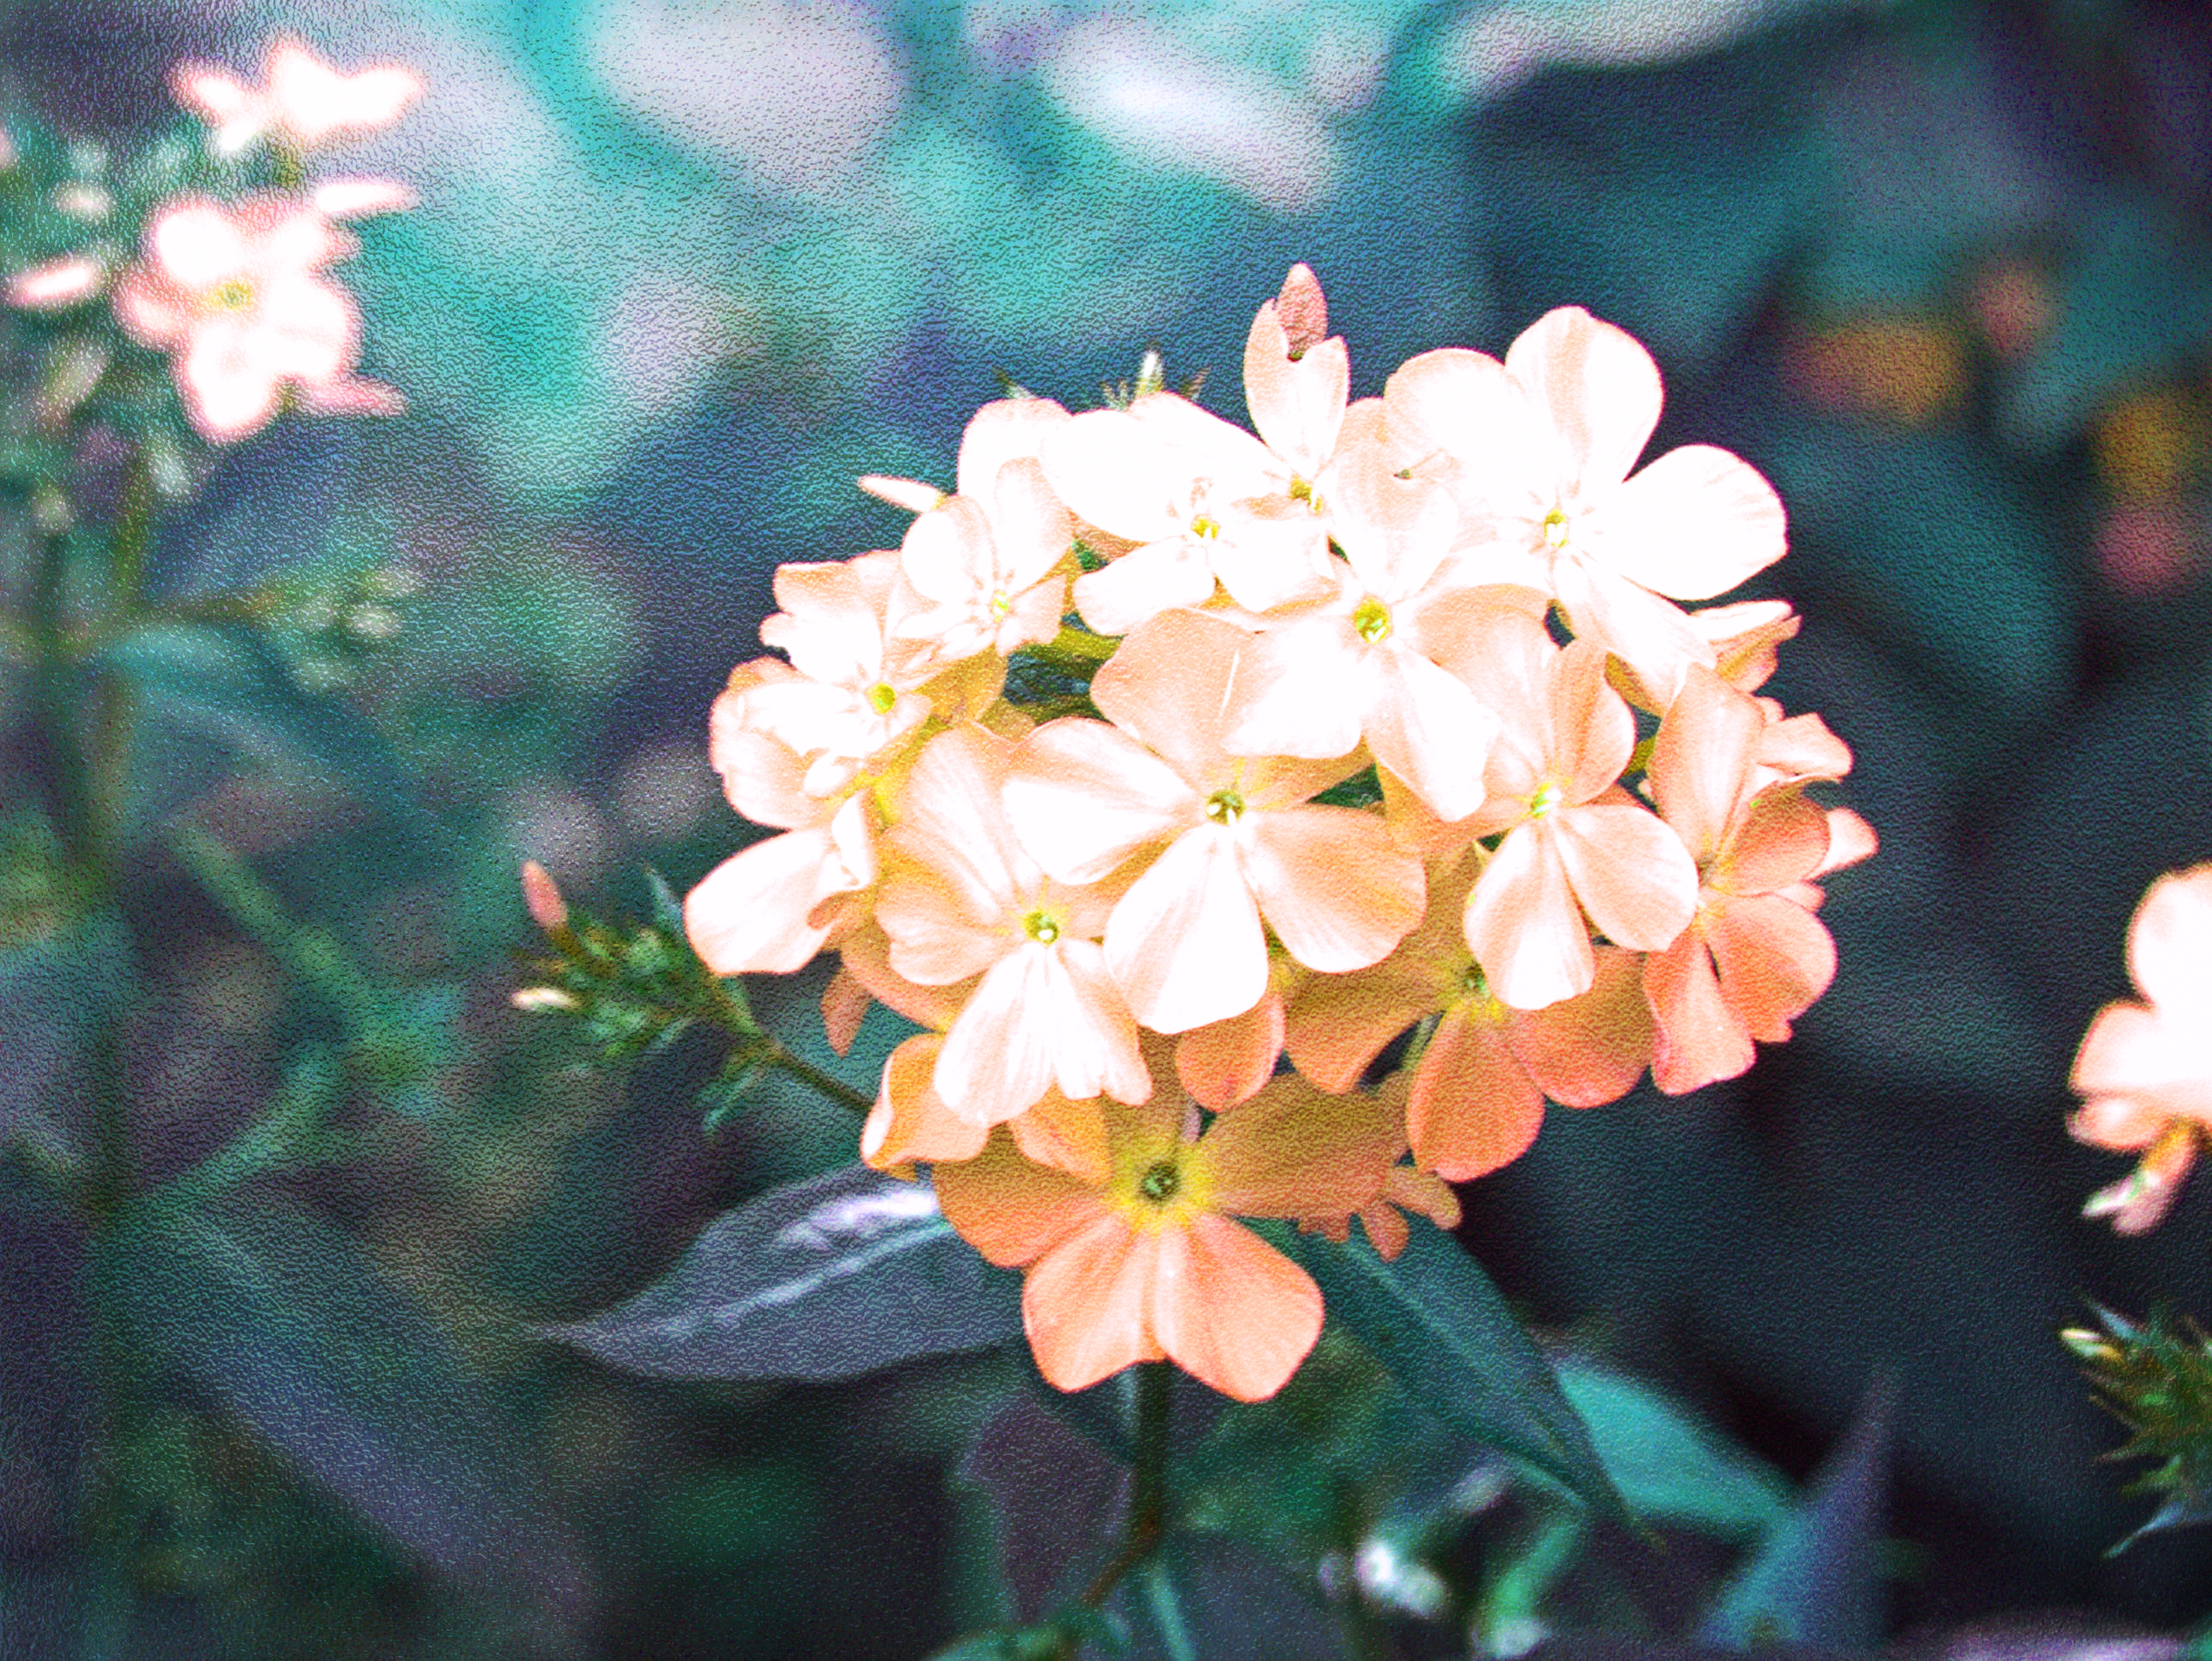
\includegraphics[width=.2\textwidth]{P1000794edit.jpg}};
\end{tikzpicture}

 % includephoto
%\end{wrapfigure}

\flushleft{\huge \bfseries Jack Kincannon}

\flushleft{\footnotesize

\faEnvelopeO \hspace{1 mm} \href{mailto:}{\tt \href{mailto:jdkincan@uark.edu}{\nolinkurl{jdkincan@uark.edu}}} \hspace{1 mm}
\faPhone \hspace{1 mm} 479-222-8082 \hspace{1 mm}
\faMapMarker \hspace{1 mm} 110 N Stadium, Fayetteville, AR \hspace{1 mm}
}
\vspace{-1em}
\flushleft{\footnotesize
\faGlobe \hspace{1 mm} \href{http://jdkincan.netlify.app}{\tt jdkincan.netlify.app}  \hspace{1 mm} 
\faTwitter \hspace{1 mm} \href{http://twitter.com/@jackkincannon}{\tt @jackkincannon} \hspace{1 mm}
\faLinkedin \hspace{1 mm} \href{https://www.linkedin.com/in/jack-kincannon-66896219b}{\tt jack-kincannon-66896219b} \hspace{1 mm}
\faGithub \hspace{1 mm} \href{http://github.com/jdkincan}{\tt jdkincan} \hspace{1 mm}
}

\begin{column}{0.60\textwidth}

\hypertarget{professional-experience}{%
\section{Professional Experience}\label{professional-experience}}

\hypertarget{tutor-current}{%
\subsection{\texorpdfstring{\textbf{Tutor
(Current)}}{Tutor (Current)}}\label{tutor-current}}

Do College Better --- Fayetteville, Arkansas

\begin{itemize}
\tightlist
\item
  Teach various subjects including: Data Analysis,~\\
  Business Law, and Finite Mathematics.
\item
  Maintain a growth mindset toward student~\\
  learning and teaching practice.
\item
  Design and facilitates differentiated and~\\
  personalized learning goals and activities.
\end{itemize}

\hypertarget{census-enumerator-2020}{%
\subsection{\texorpdfstring{\textbf{Census Enumerator
(2020)}}{Census Enumerator (2020)}}\label{census-enumerator-2020}}

US 2020 Census --- Fayetteville, Arkansas

\begin{itemize}
\tightlist
\item
  Trained and sworn in as a federal employee, aware~\\
  of all relevant statues and regulations.
\item
  Worked in a fluid environment that prioritized~\\
  teamwork and communication.
\end{itemize}

\hypertarget{caretaker-2019}{%
\subsection{\texorpdfstring{\textbf{Caretaker
(2019)}}{Caretaker (2019)}}\label{caretaker-2019}}

FS Athletic Club --- Fort Smith, Arkansas

\begin{itemize}
\tightlist
\item
  Maintained and operated equipment for a 7-acre~\\
  athletic complex.
\item
  Self-paced work environment where reliability~\\
  and trustworthiness were key.
\end{itemize}

\hypertarget{leadership-and-community-involvement}{%
\section{Leadership and Community
Involvement}\label{leadership-and-community-involvement}}

\hypertarget{communications-director-current}{%
\subsection{\texorpdfstring{\textbf{Communications Director
(Current)}}{Communications Director (Current)}}\label{communications-director-current}}

Sigma Alpha Epsilon Arkansas Alpha Upsilon

\begin{itemize}
\tightlist
\item
  Manage all fraternity related public relations,~\\
  shedding a light on positives attributes of fraternity life.
\item
  Facilitated online Formal Rush 2020 through Zoom,~\\
  commended by Director of Greek Life.
\item
  Developed an all-new website to promote the fraternity and provide a
  central information source.
\end{itemize}

\end{column}

\begin{column}{0.02\textwidth}

~

\end{column}

\begin{column}{0.38\textwidth}

\hypertarget{education}{%
\section{Education}\label{education}}

\hypertarget{b.s.-in-data-science}{%
\subsection{\texorpdfstring{\textbf{B.S. in Data
Science}}{B.S. in Data Science}}\label{b.s.-in-data-science}}

\hypertarget{finance-minor}{%
\subsection{\texorpdfstring{\textbf{Finance
Minor}~}{Finance Minor~}}\label{finance-minor}}

University of Arkansas --- Fayetteville \emph{Honors Program} GPA 4.0

\hypertarget{technical-skills}{%
\section{Technical Skills}\label{technical-skills}}

\begin{itemize}
\tightlist
\item
  Programming: Python, R, TeX,~\\
  PowerShell, Bash, RStudio, Visual Studio Code, and Microsoft Office
  Suite.
\item
  Data: importation, manipulation, transformation, visualization, and
  communication.
\item
  Managing Project Environments
\item
  Advanced Quantitative Analysis
\item
  Complex Problem Solving
\end{itemize}

\hypertarget{awards-and-distinctions}{%
\section{Awards and Distinctions}\label{awards-and-distinctions}}

\begin{itemize}
\tightlist
\item
  Chancellor's Community~\\
  Scholarship
\item
  Governor's Distinguished~\\
  Scholarship
\item
  Chancellor's List
\item
  DAR Good Citizen
\end{itemize}

\hypertarget{community-involvement}{%
\section{Community Involvement}\label{community-involvement}}

\hypertarget{sack-lunch-volunteer-current}{%
\subsection{\texorpdfstring{\textbf{Sack Lunch Volunteer
(Current)}}{Sack Lunch Volunteer (Current)}}\label{sack-lunch-volunteer-current}}

\begin{itemize}
\tightlist
\item
  Prepare and serve meals to those in need.
\item
  Adapted to COVID-19 protocols and continued to help serve my hometown.
\end{itemize}

\end{column}

\end{document}

